\chapter{Feature Combination and Dependence Investigations}
This chapter I will be:
\begin{itemize}
  \item Creating some toy tasks in RLBench
  \item Propse methods of imitiation learning to solve these tasks
  \item Experiment with the strengths and weaknesses of said methods
  \item Augment my proposals with findings
  \item Use learnings to guide proposed active policies in the next chapter \todo{maybe remove this}
  
  \todo{there are commented notes from earlier here, might help the next section}
  % \item a good vision score policy without intrinsic information about the simulator.
  %   \item simple colour checking with a threshold?? -> shit but all that I could get working 
  %   \item  reay projectrion and checking if it lands on target
  %     \item  prior info about target?? -> using CAD models I can do RBG(-D) pose estimation
  %     \item extract prior information form demonstration?
  % \item segmentation masks to pull bits out
  %   \item  How do we know which segmentation mask is my target?
  \item 
\end{itemize}


\todo{in the vision experiments section add the condlusion from `plots.ipynb'  talk about why wrist is not generalising and the possible fixes by adding depth, }


\todo{move the depth interfacing here}
% Start
\section{Increasing the Toy Task Complexity}\todo{titles may need changing in this section}

\section{Reaching with an Obstacle}
So, to carry this investigation to the next level I introduced an obstacle placing mechanism as well as randomly placing the target behind the obstacle. This is to ensure that the agent doesn't learn where the target can be behind a wall from where the obstacle is. See Figure \ref{fig:reach-obs-random} for how this task looks and the check \todo{add appendix link} for the backend wiring of these tasks.

There are two versions of this task, I thought it might be interesting to randomise the object firstly dependently then independently on the obstacle. The `dependent' randomisation called \verb|ReachObs_Random| samples the obstacle, which in turn controls the spawn boundary of where the target can spawn in, meaning the target will always appear behind the obstacle albeit, edges of it can sometimes stick out. Conversely, the `independently' random version, called \verb|ReachObs_IndRandom|, this keeps the target spawn boundary fixed, meaning the target can be anywhere in the visible workspace, but it is not necessarily always covered by the obstacle. I can see that this potentially can be useful to keep the dataset a bit more diverse, and allow the wrist camera initially observe the target sometimes.

\begin{figure}[htpb] % htpb allows all placement
  \centering
  \begin{subfigure}{0.3\linewidth}
    \centering
    \includegraphics[scale=0.3]{../fyp/assets/task-pics/reach-obs/random-front.png}
    \caption{Front}
  \end{subfigure}
  \hfill
  \begin{subfigure}{0.3\linewidth}
    \centering
    \includegraphics[scale=0.3]{../fyp/assets/task-pics/reach-obs/random-side.png}
    \caption{Side (Left)}
  \end{subfigure}
  \hfill
  \begin{subfigure}{0.3\linewidth}
    \centering
    \includegraphics[scale=0.3]{../fyp/assets/task-pics/reach-obs/random-top.png}
    \caption{Top}
  \end{subfigure}
  \vfill
  \begin{subfigure}{0.45\linewidth}
    \centering
    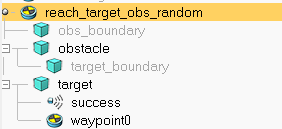
\includegraphics[scale=0.5]{assets/early-work/obs-random-scene-hierarchy.png}
    \caption{`ReachObs\_Random' Scene Hierarchy}
  \end{subfigure}
  \hfill
  \begin{subfigure}{0.45\linewidth}
    \centering
    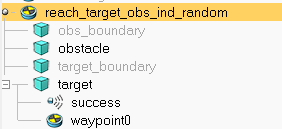
\includegraphics[scale=0.5]{assets/early-work/obs-ind-random-scene-hierarchy.png}
    \caption{`ReachObs\_IndRandom' Scene Hierarchy}
  \end{subfigure}
  \caption{Reaching Task with an Obstacle}\label{fig:reach-obs-random}
\end{figure}


\subsubsection{Wrist Camera Alone isn't Enough}

As expected, this is where the single wrist camera started showing its shortcomings. 

\todo{add graph of going around the obstacle but not quite reaching the target (wrist)}
\todo{show this with other combinations of cameras, comment on if the l/r without wrist can learn to go around the obstacle easily? maybe not, generalisation might be hard with no wrist}

The agent would easily move around the obstacle, however, would struggle to make the last steps in touching the target. This is mostly due to the fact that the demonstrations (which are provided by RLBench) are not necessarily pointing the wrist of the robot and hence the camera mounted there to look towards the target. This means that the wrist camera alone does not necessarily move towards the target, rather the robot learns to move behind the obstacle and nothing else.

From experiments I have realised that it learns to move around the obstacle easily, using simple behavioural cloning. However, getting the last nudge to actually reach the target is where it falls apart, especially in more realistic scenarios where the target is randomised behind the obstacle.

\subsubsection{Other Cameras}
Introducing the other cameras placed around in the environment, such as the \verb|left shoulder| or the \verb|right shoulder| cameras we can confirm that the wrist camera alone is not sufficient \todo{insert figure here with wrist vs others }, and the combination of wrist and other cameras are almost always the best as more coverage of the workspace guarantees less occlusions and more information the agent can work with to make decisions. It was clear that the wrist camera alone wasn't going to cut it unless it learnt to look towards the target.

\subsubsection{Implementing `Looking' into the Demonstrations}\todo{haven't done this yet}\label{ew-looking-at-target}
issues this is not easy might be working on this as a part of approach 2 later
Another solution might be to experiment with the demonstration system to make sure we are pointing the wrist camera (so, the hand of our robot) towards its target as a demonstration trajectory is calculated \todo{explain that this proved tricky and might not even be worth it}

If we can't implicitly encode the `looking' information through the demonstration that means we will have to inject this information into our agent some other way. Another way to make sure agent understands to look at the target is teaching it to actively seek out its target, either following previous works such as \todo{find some prior info tracking works add ref} where object priors are incorporated into the learning or with attention mechanisms that figure out what is important in a task without prior object information \todo{maybe reference this later}.  

\section{Expanding the Task Space: Grasping Tasks}
Another task which is likely to suffer from lack of viewpoints is a grasping task. So I designed these tasks around the idea of grasping. Firstly, a simple version (Figure \ref{fig:grasp-simple}) which the agent learns to reach then grasp the cubic target. 

Main differences between this and the reaching task is that the target here is tangible, so on top of being rendered it is also set to be \emph{collidable}. Another major addition is the usage of the \emph{extension string} as seen in \ref{subfig:simple-zoom-actions}, this instructs the demonstration engine to insert certain moves within the movement of the simple trajectory. In this case \verb|open_gipper()| ensures the gripper is open, then a later waypoint will instruct it to close.

\todo{maybe some experiment resutls here?}

The more complicated counterpart, shown in Figure \ref{fig:grasp-move}, is a scenario where the cube needs to be picked up then moved to the target location (designated in green)

\begin{figure}[htpb] % htpb allows all placement
  \centering
  \begin{subfigure}{0.3\linewidth}
    \centering
    \includegraphics[scale=0.2]{../fyp/assets/task-pics/grasp/simple-front.png}
    \caption{Front}\label{subfig:simple-front}
  \end{subfigure}
  \hfill
  \begin{subfigure}{0.5\linewidth}
    \centering
    \includegraphics[scale=0.3]{../fyp/assets/task-pics/grasp/simple-front-zoom-gripper_actions.png}
    \caption{Zoomed, with gripper action}\label{subfig:simple-zoom-actions}
  \end{subfigure}
  \caption{Simple Grasping Task}\label{fig:grasp-simple}
\end{figure}

\begin{figure}[htpb] % htpb allows all placement
  \centering
  \begin{subfigure}{0.45\linewidth}
    \centering
    \includegraphics[scale=0.2]{../fyp/assets/task-pics/grasp/move-front.png} 
    \caption{Front}\label{subfig:grasp-move-front}
  \end{subfigure}
  \hfill
  \begin{subfigure}{0.45\linewidth}
    \centering
    \includegraphics[scale=0.2]{../fyp/assets/task-pics/grasp/move-top.png}
    \caption{Top}\label{subfig:grasp-move-top}
  \end{subfigure}
  \caption{Grasping then moving}\label{fig:grasp-move}
\end{figure}


\missingfigure{grasp pic and possibly the demo gifs, }
\todo{add a picture with the cube grasped and the wrist camera view seen at that point}
Although, initially the wrist camera shouldn't pose any problems, as we advance through the task, especially after we have grasped something the wrist mounted camera becomes heavily obstructed and becomes unreliable so basing our decisions on this medium alone is not ideal.

\subsubsection{Observations}
What I got from these experiments was that the agent can benefit from understanding its surroundings at a higher level and more importantly remembering them. This is because once the camera becomes obstructed, as with \emph{Grasp Then Move}, even if the agent could do some exploration to find the target, it wouldn't be ideal due to the restricted view it has access to. So, observing the environment before, and remembering important parts will be vital for the later stages of tasks. I aim to explore some pre-policy visual exploration of the environment to be albeit to address issues such as this one.

\section{}
% Depth Interfacing
\section{Camera Dependence Investigations}\todo{does this warrant a whole new section or should I talk about it within obs and no-obs and grasp etc}
Following on from the earlier discoveries I wanted to dig deeper into the importance of different camera views and different sensors.

\subsection{Depth Interfacing} \todo{this is not done yet, gonna be a long week init}
\section{Depth Interfacing}
Another area of important research, before relating all this back to active vision, is figuring out distance. Depth interfacing is an important part of perception. Continuing from the drawn parallels to humans, we place object in our fields of vision by our two eyes. Stereo-vision, allows us to process two slightly different poses of a target object to reinforce our understanding of where that object is in the environment around us. Other information such as lighting (and shadows) may unconsciously help us as well. The main takeaway is that understanding distance to an object goes a long way in firstly understanding how to approach an object.

There are a few ways to achieve this in robotics. In RLBench specifically is either to use two cameras (with a known distance between the two cameras to adjust poses with known intrinsics). However, RGB cameras are not the only things we have access to. We also we have a depth sensor.

This is because, as I hinted earlier in the background section, the main idea of active vision is to be able to use minimal amounts of viewpoints and make the most out of these. In this scenario, I want to see if it can be justified to use the wrist camera accompanied by the wrist depth sensor to replace any other cameras we might have around the workspace. Paving the way to the next section in proposing active vision policies that act solely on information from a repositionable sensor.

Therefore, it is important to study shortcomings of individual sensors with respect to others to understand how policies with limited access to sensors can be made to overcome such challenges without necessarily adding more points of observability to a workspace.

\subsection{Grasping with Varying Depths}
To start investigating, I devised the following test task to see how the agent reacts to differently sized targets that might be placed at varying distances from the gripper within the scene

\subsubsection{Task Design}
A grasping task makes sense for this experiment. Because unlike the reaching tasks from earlier, the robot will need slightly more precision in executing its grasp and actually grabbing the target. The task performer needs to figure out where an object is before attempting to grab it. So, I created a modified version of the simple grasping task where the target object's distance and scale can be externally varied to observe the behaviours of agents in a controlled manner.\todo[color=green]{talk about delegating the task creating and param passing as well as the tasks in appendix and link here}

\begin{figure}[htpb] % htpb allows all placement
  \centering
  \begin{subfigure}{0.4\linewidth}
    \centering
    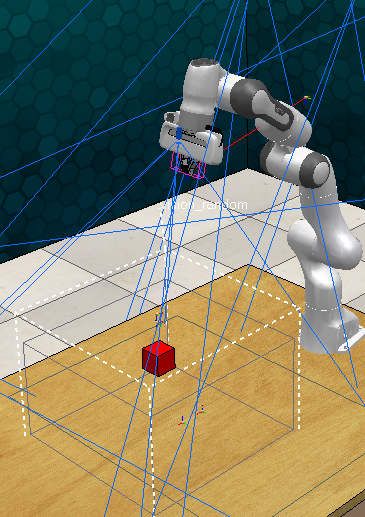
\includegraphics[width=0.7\linewidth]{assets/depth-interfacing/normal-size-grasp.png}
    \caption{Normal Target Size}\label{subfig:normal-grasp}
  \end{subfigure}
  \begin{subfigure}{0.4\linewidth}
    \centering
    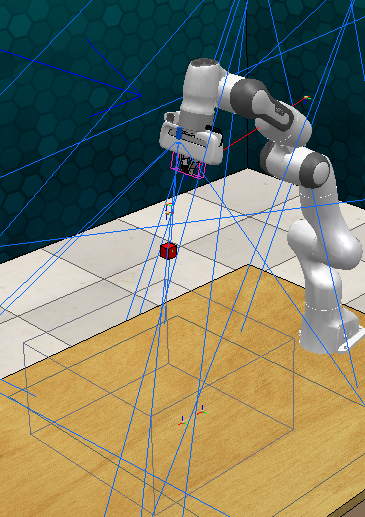
\includegraphics[width=0.7\linewidth]{assets/depth-interfacing/smaller-grasp.png}
    \caption{Smaller Target Size}\label{subfig:small-grasp}
  \end{subfigure}
  \caption{Visualisation of the Depth Interfacing experiment task}\label{fig:di-task}
\end{figure}

Figure \ref{fig:di-task}, is the general setup I am planning on using to evaluate the depth sensor versus a multi-view setup. Initial observations from the side clearly indicate that these are two different targets and will require different reach lengths before the agent can attempt to grab them.

\begin{figure}[htpb] % htpb allows all placement
  \centering
  \begin{subfigure}{0.4\linewidth}
    \centering
    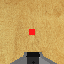
\includegraphics[width=0.7\linewidth]{assets/depth-interfacing/normal-size-wrist.png}
    \caption{Smaller - Wrist RGB}\label{subfig:normal-rgb}
  \end{subfigure}
  \begin{subfigure}{0.4\linewidth}
    \centering
    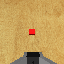
\includegraphics[width=0.7\linewidth]{assets/depth-interfacing/smaller-wrist.png}
    \caption{Smaller - Wrist RGB}\label{subfig:small-rgb}
  \end{subfigure}
  \begin{subfigure}{0.40\linewidth}
    \centering
    
\includegraphics[width=0.7\linewidth]{assets/depth-interfacing/normal-depth.png}
    \caption{Wrist Depth Mask - Normal}\label{subfig:normal-depth}
  \end{subfigure}
  \begin{subfigure}{0.40\linewidth}
    \centering
    
\includegraphics[width=0.7\linewidth]{assets/depth-interfacing/smaller-depth.png}
    \caption{Wrist Depth Mask - Smaller}\label{subfig:small-depth}
  \end{subfigure}
  \caption{Wrist RGB and Depth Masks for the tasks}\label{fig:di-rgb-vs-depth}
\end{figure}

However, as seen in the comparison in \ref{subfig:normal-rgb} and \ref{subfig:small-rgb}, the RGB outputs look practically the same, and will very likely produce extremely similar features after extraction. A way to differentiate them would be to utilise the wrist depth mask in this encoding. As shown in \ref{subfig:normal-depth} and \ref{subfig:small-depth}, they now carry different features in those areas. In the depth mask the darker colours indicate closer objects, and the information is encoded as floats. 

\begin{figure}[htpb] % htpb allows all placement
  \centering
  \begin{subfigure}{0.40\linewidth}
    \centering
    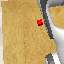
\includegraphics[width=0.7\linewidth]{assets/depth-interfacing/normal-l_rgb.png}
    \caption{Normal - Left Shoulder RGB}\label{subfig:normal-l-shoulder}
  \end{subfigure}
  \begin{subfigure}{0.40\linewidth}
    \centering
    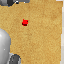
\includegraphics[width=0.7\linewidth]{assets/depth-interfacing/normal-r_rgb.png}
    \caption{Normal - Right Shoulder RGB}\label{subfig:normal-r-shoulder}
  \end{subfigure}
  \begin{subfigure}{0.40\linewidth}
    \centering
    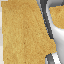
\includegraphics[width=0.7\linewidth]{assets/depth-interfacing/smaller-l_rgb.png}
    \caption{Smaller - Left Shoulder RGB}\label{subfig:smaller-l-shoulder}
  \end{subfigure}
  \begin{subfigure}{0.40\linewidth}
    \centering
    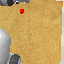
\includegraphics[width=0.7\linewidth]{assets/depth-interfacing/smaller-r_rgb.png}
    \caption{Smaller - Right Shoulder RGB}\label{subfig:smaller-r-shoulder}
  \end{subfigure}
  \caption{Left and Right Shoulder RGB Cameras}\label{fig:di-lr-shoulder}
\end{figure}


Another possible differentiating factor, and the reason earlier tasks were performing well, is due to the shoulder cameras. These also provide extra information about the scene the agent can use to understand its 3D geometry, even if it isn't explicitly taught. Although these are also not perfect, as seen in \ref{subfig:smaller-l-shoulder}, this camera is completely obstructed by the robot and is not seeing the target. This is not immediately problematic, because a smart enough system might be able to reason that the target is visible on the right and not on the left, leading to devising the correct depth for it. However, I have not intentionally encoded that information and doubt this network will be able to produce correct results with these observations.

\subsubsection{Adding Stereo Wrist Vision}\todo[color=blue]{can be removed not sure}
A possibility to overcome this \emph{self-occlusion} is to introduce stereo vision at the wrist level. Adding 2 off-centre cameras to the gripper, likely to the left and right of the existing wrist camera, will fix the self-occlusion, and possibly create a better comparison to the \emph{Wrist RGB} and \emph{Wrist Depth} combination. However, this comes with a lot of rewiring of RLBench and with its likely hidden issues that will pop up later. I did not want to take on this large architectural change before continuing with main investigation of the project, however, if timings permit this will be an important addition to the testing suite.


